\documentclass{article}

\usepackage{amsmath}

\usepackage{mathptmx}           
\usepackage{graphicx}           
\usepackage{url}            
\usepackage{subcaption}    

\usepackage[a4paper,margin=2cm]{geometry}

\usepackage{natbib} 
\usepackage[numbered, framed]{mcode}

\usepackage{lipsum}

\begin{document}

\author{H. Blum, D. Cavezza, A. Paudice and M. Rohbeck\\
 Machine Learning CO395\\
  Imperial College London}
\date{\today}
\title{Assignment 2: Decision Trees Algorithm}
\maketitle

\begin{abstract}
\lipsum[5]
\end{abstract}

\section{Implementations}
From the set of 6 Decision Trees, each tree will return a binary classification for a given data sample. Therefore, we need an Algorithm that decides on Basis of the output of the 6 trees, which class the given sample falls into. In fact, this algorithm does not even have to depend on the output of the classification trees. For example, one could think of an algorithm that simply outputs a randomly choosen classification and will have an accuracy of 17\% for a balanced test set. However, we searched for algorithms with a better performance.


\subsection{Stacking}
As we already implemented the basis function to train a decision tree, we tried to approximate the decision function (the function which outputs a class for a given example) by another tree which is trained on basis of the output of all 6 binary classification trees for the training set.
Therefore, given a sample, the decision algorithm works as follows:
\begin{enumerate}
    \item give the sample to the 6 binary classification trees
    \item give the output of all 6 trees to the decision function tree and output it's output
\end{enumerate} 

\subsubsection{Statistics}
The stacked tree method achieves a general accuracy of 72.4\% on clean data and 58.8\% in noisy data.

\begin{figure}[h]
    \hspace*{\fill}%
    \subcaptionbox{confusion matrix for clean data}{
        $\begin{bmatrix} 105 & 9 & 2 & 1 & 9 & 6\\ 37 & 145 & 1 & 5 & 3 & 7\\ 21 & 4 & 79 & 1 & 4 & 10\\ 13 & 10 & 4 & 177 & 5 & 7\\ 39 & 13 & 3 & 6 & 64 & 7\\ 18 & 5 & 13 & 6 & 8 & 157 \end{bmatrix}$
    }\hfill%
    \subcaptionbox{performance for the different classes with clean data}{
        \begin{tabular}{c | c c c}
        Class & Precision & Recall & $F_1$ \\
        \hline \hline
        1 & 48.3\% & 79.6\% & 57.6\% \\ 
        2 & 78.5\% & 73.7\% & 75.5\% \\ 
        3 & 76.5\% & 64.9\% & 69.8\% \\ 
        4 & 90.4\% & 82.5\% & 86.0\% \\ 
        5 & 66.3\% & 47.6\% & 54.7\% \\ 
        6 & 85.8\% & 76.4\% & 79.7\% \\ 
        \end{tabular}
    }%
    \hspace*{\fill}
    \\
    \hspace*{\fill}%
    \subcaptionbox{confusion matrix for noisy data}{
        $\begin{bmatrix} 19 & 7 & 16 & 4 & 9 & 33\\ 13 & 130 & 7 & 8 & 2 & 27\\ 13 & 16 & 98 & 11 & 4 & 45\\ 10 & 14 & 13 & 141 & 1 & 30\\ 21 & 8 & 4 & 6 & 43 & 28\\ 13 & 8 & 21 & 9 & 11 & 158  \end{bmatrix}$
    }\hfill%
    \subcaptionbox{performance for the different classes with noisy data}{
        \begin{tabular}{c | c c c}
        Class & Precision & Recall & $F_1$ \\
        \hline \hline
        1 & 23.5\% & 21.6\% & NaN\% \\ 
        2 & 70.2\% & 68.1\% & 68.8\% \\ 
        3 & 60.8\% & 51.1\% & 54.8\% \\ 
        4 & 78.1\% & 67.6\% & 72.0\% \\ 
        5 & 59.9\% & 38.1\% & 45.4\% \\ 
        6 & 49.1\% & 71.8\% & 57.7\% \\ 
        \end{tabular}
    }%
    \hspace*{\fill}
    
    \caption{statistics of the stacked tree}
\end{figure}





\subsection{Probabilistic Trees}
In this implementation, we assign a score to each leaf of every tree between 0 and 1. The score is correlated to the number of training examples that can be classified by the given leaf with respect to the total number of training examples in every class.
\begin{align*}
    \textrm{score} = \frac{\textrm{\# correctly classified training data by this leaf}}{\textrm{\# training data in this tree}}
\end{align*}
Of all binary classification trees returning 1, the decision algorithm will pick the class corresponding to the tree with the highest decision score. If no tree returns 1, it will pick at random.
\begin{lstlisting}
function [ predictions ] = decide_by_score(trees, testset)
% decide_by_score performs a classification based on the fraction of
% correctly classified training examples given by the tree leafs

[m,n] = size(testset);
predictions = zeros(m,1);

for i = 1:m
    % test in all trees, find the one with the best score
    best_score = 0;
    predictions(i) = NaN;
    for t = 1:6
        [pred, score] = prediction_with_score(trees(t),testset(i,:));
        if pred == 1
            % the tree recognises this item as his class
            if score > best_score
                predictions(i) = t;
                best_score = score;
            end
        end
    end
    % If all the predictions are 0, pick a random class
    if(isnan(predictions(i)))
        predictions(i) = randi(6);
    end
end

end
\end{lstlisting}


\subsubsection{Statistics}
The described method achieves a general accuracy of 73.2\% on clean data and 64.4\% in noisy data.

\begin{figure}[h]
    \hspace*{\fill}%
    \subcaptionbox{confusion matrix for clean data}{
        $\begin{bmatrix} 88 & 15 & 7 & 4 & 11 & 7\\ 15 & 145 & 5 & 7 & 14 & 12\\ 7 & 5 & 83 & 2 & 5 & 17\\ 4 & 8 & 6 & 188 & 5 & 5\\ 15 & 19 & 2 & 10 & 73 & 13\\ 3 & 9 & 14 & 11 & 4 & 166 \end{bmatrix}$
    }\hfill%
    \subcaptionbox{performance for the different classes with clean data}{
        \begin{tabular}{c | c c c}
        Class & Precision & Recall & $F_1$ \\
        \hline \hline
        1 & 66.3\% & 63.1\% & 63.4\% \\ 
        2 & 72.4\% & 75.1\% & 73.3\% \\ 
        3 & 67.1\% & 65.9\% & 66.2\% \\ 
        4 & 79.1\% & 84.0\% & 81.0\% \\ 
        5 & 60.5\% & 55.1\% & 57.5\% \\ 
        6 & 83.3\% & 81.1\% & 82.0\% \\
        \end{tabular}
    }%
    \hspace*{\fill}
    \\
    \hspace*{\fill}%
    \subcaptionbox{confusion matrix for noisy data}{
        $\begin{bmatrix} 21 & 11 & 20 & 8 & 19 & 9\\ 16 & 132 & 13 & 15 & 6 & 5\\ 14 & 13 & 108 & 22 & 11 & 19\\ 8 & 13 & 10 & 161 & 10 & 7\\ 15 & 10 & 8 & 7 & 59 & 11\\ 13 & 9 & 14 & 10 & 10 & 164 \end{bmatrix}$
    }\hfill%
    \subcaptionbox{performance for the different classes with noisy data}{
        \begin{tabular}{c | c c c}
        Class & Precision & Recall & $F_1$ \\
        \hline \hline
        1 & 25.5\% & 23.3\% & NaN \\ 
        2 & 71.4\% & 69.7\% & 69.9\% \\ 
        3 & 64.4\% & 56.7\% & 59.2\% \\ 
        4 & 71.6\% & 77.6\% & 74.0\% \\ 
        5 & 51.0\% & 52.9\% & 50.7\% \\ 
        6 & 76.2\% & 74.1\% & 74.6\% \\
        \end{tabular}
    }%
    \hspace*{\fill}
    
    \caption{statistics on the probabilistic tree}
\end{figure}


\section{Pruning}
\begin{figure}
\centering
\subcaptionbox{Pruning Example with clean data}{
    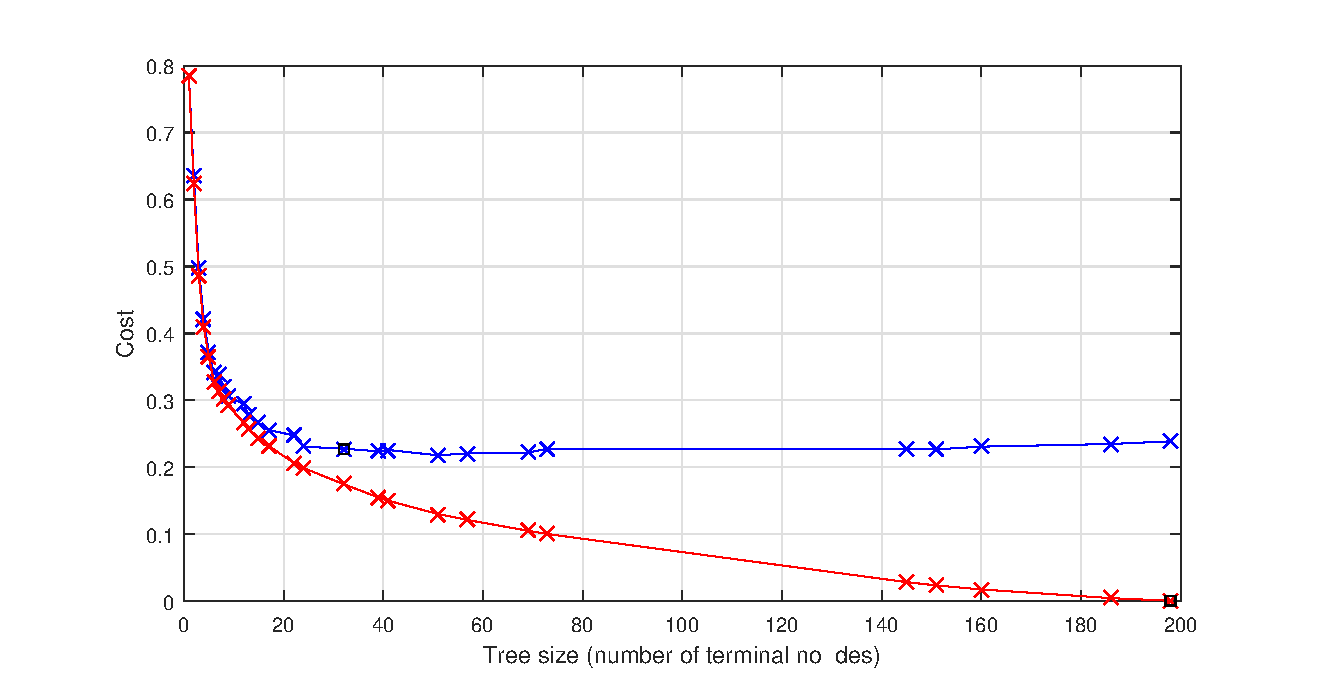
\includegraphics[scale=.4]{pruning_clean_data.eps}
}
\subcaptionbox{Pruning Example with noisy data}{
    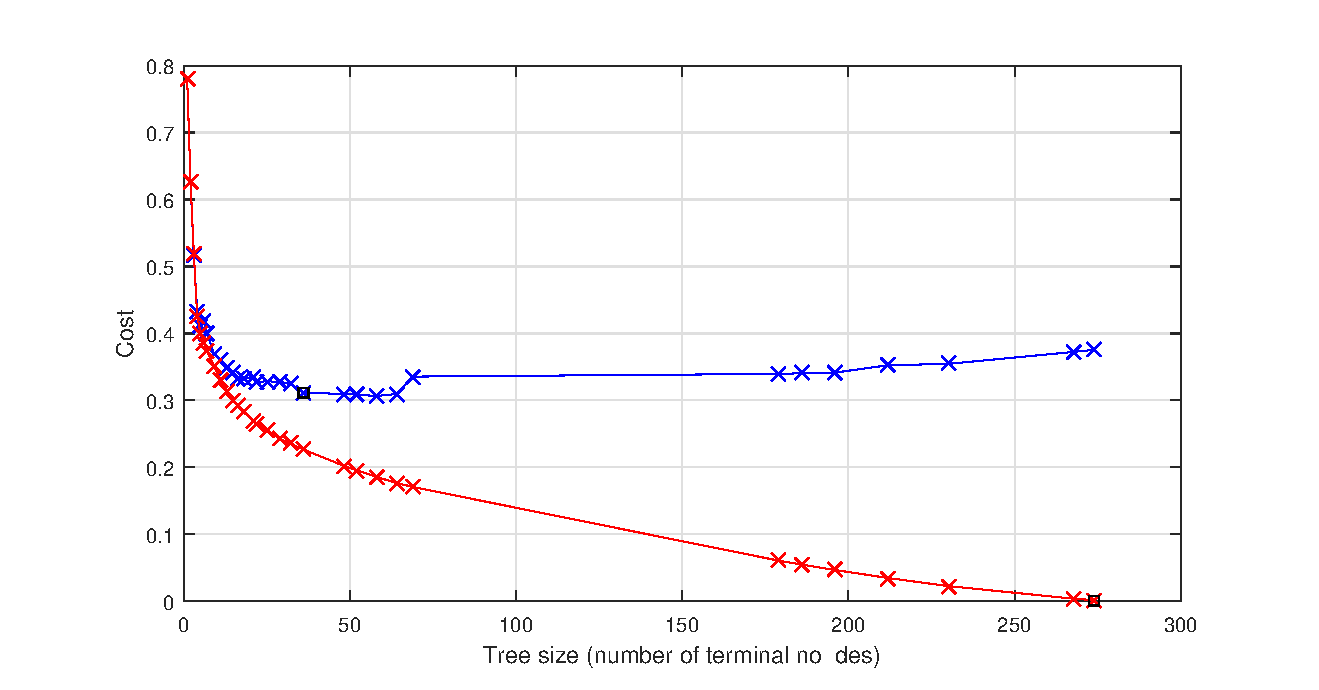
\includegraphics[scale=.4]{pruning_noisy_data.eps}
}
\end{figure}

These Figures show the error rate on validation and training set as the size (i. e. the number of leaves) of the trees increase.
For clean data the actual loss in accuracy is, as can be seen, negligible. With the optimal size, the error rate is 21\% instead of 24\% with no pruning.\\
For noisy data, this difference becomes much bigger. Pruning can increase performance in this case by approx. 10\% from 62\% to 68\%.

\section{Performance with Noisy Data}
The Performance with noisy data is much worse. Decision Trees can represent any kind of function, also the function generating noise. This is because while training the decision trees, we fit our tree to the training data, even if this data is noisy. Therefore noisy data generates noisy trees.
For Class 1 (precision is less than half in comparison to clean data) we especially have a problem of overfitting wich leads to much worse precision than with the clean data.

\section{Choosing the Best Algorithm}
We tested each of our algorithms using cross-validation. The Accuracy on the cross-validation test set is at this point a valid approximation of the accuracy on the unknown data set. On basis of these approximations, we choose the algorithm with the best accuracy.
After choosing an algorithm, we train it with the whole data set we got. Unfortunately, we don't have a test set to estimate the performance of this trained algorithm on unseen data.

\bibliographystyle{plainnat}
\bibliography{example}

\end{document}
